\documentclass[]{article}
\usepackage{amssymb,amsmath}

\usepackage[style=verbose]{biblatex}
\addbibresource{biblio.bib}

\usepackage{pdflscape}

\usepackage{fontspec}
\defaultfontfeatures{Ligatures=TeX,Scale=MatchLowercase}
\setmainfont[]{cantarell}

\usepackage{graphicx}
\usepackage{wrapfig}
\usepackage{hyperref}
\urlstyle{same}  % don't use monospace font for urls
\usepackage[margin=4pt]{subcaption}

\usepackage[margin=2cm]{geometry}
\usepackage{longtable,booktabs}

\usepackage{pgfgantt}
\usepackage{rotating}

\usepackage{tocloft}

\renewcommand{\thesubsubsection}{}

\usepackage{xspace}
\newcommand{\project}{WizMe\xspace}

\newcommand{\task}[2]{\vspace{0.5cm}\noindent\emph{Task T#1}: {\bf #2}\par}

\newcommand{\D}[3]{\emph{Deliverable D#1} (M#2): #3\\}

\newcommand{\TODO}[1]{{\color{red}\textbf{TODO: #1}}}

\newcommand{\severin}[1]{{\color{red}\textbf{Severin: #1}}}
\newcommand{\toseverin}[1]{{\color{red}\textbf{To Severin: #1}}}
\newcommand{\eu}[1]{{\color{teal}\textbf{Guidelines EU ERC: #1}}}
\newcommand{\cellgrey}{\cellcolor[gray]{0.85}}


\title{\project - Part B}

\begin{document}
\maketitle

\subsection{Notes}

\paragraph ACAMH conference on Mental health and refugees:

Keywords:
\begin{itemize}
    \item Trauma
    \item Unaccompanied Asylum Seeking Children
\end{itemize}

Discussion with Helen Peden, Refugee Council, happy to contact
\begin{itemize}
    \item litteracy issues; example -> learn to read a map
    \item need to be primarily verbal
    \item work with 16/20 yo

\end{itemize}

\begin{itemize}
    \item 25M refugees, 50\% under 18
\end{itemize}

Good talk b Sarah Hunt (Uni Leicester)

\begin{itemize}
    \item Participatory Action Research ("From voice to agency", Rodriguez and
        Brown 2009)
    \item focus on post-migratory risk factors to mental health
    \item hceck photo of litterature review
    \item check participatory methodology (photos of slides)
    \item 3 themes emerging from her research: understanding trauma; need for
        responsive/individualised pathways; need for housing + basic needs
        provisions
    \item she mention lack of privacy in some provided housing as a permanent
        threat and a source of stress/trauma: \textbf{relation to privacy by
        design}
    \item point out the need to support not only the children but also the
        schools
    \item reference to World Awarness Children in Trauma Model (WACIT, Vostanis
        2012-2018)
    \item example of social integration issues: lack of knowledge of school
        rules (like raising ones' hands, perceived as bad behaviours/threatening
        behaviour); difficulty to meet with peers
    \item point raised about need for refugee children to 'fit in a new
        identity, matching local norms/expectation, at the cost of the previous,
        original identity -> source of suffering: importance of \emph{securing
        identity}, as done by some schools (example of school inviting parents
        of diverse background to come and cook home dishes at school, with
        different background every week)
\end{itemize}


Prof Ravi Kohli (child welfare):

\begin{itemize}
    \item Safety <-> belonging <-> success (cf photo)
    \item ...but not a straight line! Comes and go!
    \item underline the need by refugees to reciprocate
    \item make a strong point on individual identities instead of being just a label (cf
        photo)
    \item \textbf{importance of individual stories}
\end{itemize}

Powerful presentation by Bobby Lloyds; she stayed 2 days/week for 4 years in
Calais camp; visual artist + art therapist; large archive of field experience on
Facebook account (ArtRefuge UK)

She points out the importance of mobile phones -> communication, story telling,
etc

Talk Lucy Arnsby-Wilson:

\begin{itemize}
    \item "how can we help people to feel fully alive?"
    \item a couple of examples of cultural differences (cf photo 'Rights and
        autonomy')
    \item mental safety at the end of the interaction: "will you remember me?"
\end{itemize}

Talk Katheryn Cronin (lawyer, really interesting, might be worth contacting her
for feedback if we go the 'robot collecting stories' route)

\begin{itemize}
    \item "process if requesting refugee status is highly destructive"
    \item importance of the narration, story when facing home office/judge
    \item \textbf{robot to collect \emph{individual} stories and print them out as
        testimonies}: could be useful to help children to build up their case
    \item often the story ("dad abducted by talibans, mum fearing for child,
        send child away") is heard again and again by judges, they automatically
        dismiss it as being a lie based on a 'template' provided by smugglers
    \item the children often lack the skillset required to tell their stories as
        they come from small villages where everyone know everyone (-> no need
        to ever tell own story)
    \item children also struggle to communicate/explain misunderstandings to
        judge due to different realities: eg: no street light in Afghanistan
        village, so child could hide from taliban raid. Hard to believe for UK
        judge, but the child does not understand why it is hard to believe as he
        does not know that every single street/house would have lights in the UK
    \item she mention the type of room (light, airy, placement of chairs, etc)
        to avoid reproducing the sense of oppression experienced by the children
        during their journey (eg locked in the back of a lorry)
    \item refugee convention is about assessing vulnerability of children if
        they were to return -> most of the interviews while requesting asylum is
        about assessing/measuring weaknesses/vulnerabilities instead of their
        strength/resilience while they travelled the world. Harsh. need to
        'train' the children to talk about their vulnerabilities.
    \item 'is their story tainted by smugglers'? question of how genuine the
        story is. Use of robot to disclose their stories?
    \item example of Afgani children often told to claim their parents are dead
        or disappeared as they are told it could help them getting refugee
        status. Counter productive (because create inconsistencies in their
        stories) + traumatic
    \item importance of the sense of security <-> trust -> robot needs to by
        trustworthy \textbf{high level of privacy, control; privacy by design}
    \item under EU law, children must receive support to reconnect with their
        families, but almost nothing is done. Could robots help by sharing
        stories online? (potential privacy landfield, though)
\end{itemize}

Imran Shah: interpretation business. Might be an interesting contact if we
develop multi-lingual capabilities.

\subsection*{Title of the proposal}\label{title-of-the-proposal}

\textbf{Social robots to support human-human interactions}

\subsection*{Acronym}\label{acronym}

\project

\subsection*{Abstract}\label{abstract}

\pagebreak

%%%%%%%%%%%%%%%%%%%%%%%%%%%%%%%%%%%%%%%%%%%%%%%%%%%%%%%%%%%%%%%%%%%%%%%%%%%%%%%%%%%%%%%%
%%%%%%%%%%%%%%%%%%%%%%%%%%%%%%%%%%%%%%%%%%%%%%%%%%%%%%%%%%%%%%%%%%%%%%%%%%%%%%%%%%%%%%%%
%%%%%%%%%%%%%%%%%%%%%%%%%%%%%%%%%%%%%%%%%%%%%%%%%%%%%%%%%%%%%%%%%%%%%%%%%%%%%%%%%%%%%%%%
\section{B1.a. Extended Synopsis of the scientific proposal}\label{part1}
\eu{(max 5 pages)}

\eu{The Extended Synopsis should give a concise presentation of the scientific
proposal, with particular attention to the ground-breaking nature of the
research project and the feasibility of the outlined scientific approach.
Describe the proposed work in the context of the state of the art of the field.
References to literature should also be included. References do not count
towards the page limits. It is important that this extended synopsis contains
all essential information including the feasibility of the scientific proposal
since the panel will only evaluate Part B1 at step 1.}



\project is a future-looking project that aims at investigating how social
robots can shape and support stronger \emph{human-human} relationships. In a
time where robots are on the verge of becoming pervasive in our daily, human
environment, can we ensure 'by design' that they will become powerful tools to
foster rich, positive interactions between the people themselves, and build a
stronger, more cohesive society?

'Socially intelligent' robots require unique, beyond state-of-the-art,
capabilities to \emph{(1)} understand the social interactions (social
situation awareness), \emph{(2)} decide the best course of action for
short-term and longer-term social influence, and \emph{(3)} perform the
appropriate social actions and exert adequate, ethical social influence.

However, extreme complexity hides behind these seemingly well-delineated
technical steps: not only the technology itself is beyond state-of-the-art, but
the interplay between technology, socio-cognitive psychology, privacy and ethics
is only starting to be researched and understood. \project offers a ambitious
vision and a strong, evidenced-based, methodology to significantly advance our
understanding of this difficult question. A conceptual framework, grounded in
actual technology and field experience, to discuss and evaluated the role and
impact of social robots in tomorrow's society.




\subsection{Long-term vision and targeted breakthrough towards that vision}

While the original idea of the
'multi-function-household-robot-that-does-the-dishes' has yet to materialise --
physical manipulation of objects in an unstructured environment is hard, as it
happens --, social robots are nevertheless in the process of establishing
themselves as important tools in a variety of other situations, where they play
a key role as social agents.

As a researcher who has been working for the last 12 years in the field of
human-robot interaction, I have been both a witness and an actor of the crossing
of a critical milestone: the emergence of \textbf{durable social interactions}
between artificial intelligences embodied in robots, and humans. We have been
witnessing over the last two years an explosion of the number of studies
involving social robots, deployed in real-world settings (schools, care centres)
over relatively long periods of time (up to 2 or 3 months at a time). In most of
these experiments, robots are not fully autonomous, even though full autonomy is
in sight as well.

While many see these developments positively, or even as a turning point [...]
other express skeptism or worry that this might lead to a deshumanization of our
society. Indeed, if artificial agents are to engage into social interactions
with us, and enter as such our human 'pré carré', pressing ethical questions
need to be answered.

\begin{itemize}
    \item how to ensure that social robots are not used to simply replace humans
        (like social workers) to cut costs?
    \item can we guarantee that the use of social robots will always be ethically motivated?
    \item even further, can we implement some ethical safeguarding at the core
        of the system?
    \item what about privacy? how to trust that robots in our home or school or
        hospital will not eavedrop on our private lives?
\end{itemize}

These questions are not only legitimate, but also pressing: the recent rise of
personal assistants like Alexa or Google Home, with the major privacy concerns
that accompanied their deployments in people home, shows that letting the
industry set the agenda on these questions is not wise -- and robots can
potentially be much more intrusive than immobile smart speakers.

Social robots have two unique properties which distinguish them from these smart
speakers, and significantly complexify their conceptual framing. First, they are
fully embodied, and they physically interact with their environment, from moving
around, to picking up objects, to looking at you; second, willingly or not, they
are ascribed \emph{agency} by people.  This second difference has far-reaching
consequences, from affective bonding to over-trust, to over-disclosure of
personnal, possibly sensitive, informations [cite paper HRI children
disclosure].



This progress raises questions, both practical and more fundamental:

inventing and building a principled cognitive architecture for tomorrow's social
robots, nutrured by decades of research in understanding human social cognition,
and where ethics and privacy are intrinsic to the system.

Due to the complex interplay between the technical implementation, the
socio-psychological determinants of the interactions, and the multiple ethical
mechanisms that have to be built-in the system, it is difficult to build one
coherent and consistent perspective on the whole question. As a consequence, a
conceptual, intellectual framework emcompassing both the internal cognitive
mechanisms required by socially intelligent robots, as well as their role and
impact in the society, only exists in fragmented pieces  is essentially missing.

The lack of such a proper conceptual framing is a critical issue: for robots to
have a positive impact on the society, with strict ethical and privacy-related
safeguarding, it is urgent that the wider academic and intellectual communities,
beyond technologist, embrace this question and build up the debate on the
acceptability of robots in our society.

As such, the foundational ambitious of \project is to create a conceptual
framework around social robots in the human society, by reframing the widely
accepted, yet sorely unspecific, idea of \emph{human-robot interaction} into the
more specific idea of \emph{robot-supported human-human interactions}: the robot
is considered from the perspective of how it can \emph{support} humans, and in
particular, support stronger, positive interactions between humans.

Critically, though, \project will ground this conceptual frame into the reality
of socio-cognitive AI and real-world deployments of social robots.


\subsubsection{Three pilars}

To achieve the vision of a natural and harmonious \emph{co-habitation} between
social robots and humans, ...

The \project project will, for the first time, take a broad, holistic approach
to these questions, and as such, is build around three pilars:

\begin{enumerate}
    \item AI architecture for decision making
    \item socio-psychological design of the interaction, from 1-to-1
        interaction, to group interaction, to interaction with the eco-system
    \item built-in privacy and ethics
\end{enumerate}

The difficulty comes from the fact that these pilars do not represent independent
research questions: they are deeply woven together, in intricate ways.


Taken independently, these three pilars are already intrinsically complex.

The first pilar, AI Architecture for Decision Making, for instance:
state-of-the-art decision making processes for social robots are build from
multiple algorithmic layers: classical machine learning (like classifiers, or
SLAM) for low-level sensori-motor processing; probabilistic data processing (for
e.g. localisation or point cloud processing); deep neural networks for object
recognition, scene understanding, speech and dialogue processing; classical
symbolic reasoning (for instance, for task planning); high-level knowledge
representation and reasoning (semantic webs); hybrid spatial/symbolic reasoning
for motion planning; etc.

Importantly, these layers are not typically combined in a simple, linear
fashion: modern control architectures are distributed, loosely coupled, and
design so that information flows in multiple directions, at different levels of
abstraction, in order to create complex feedback loops, and achieve systems that are
both goal-directed \emph{and} reactive (event-driven).


The real complexity of such AI architectures is however striking when one tries
to answer \emph{how} such an architecture can enable the realisation of the
desired socio-cognitive functions, i.e. our second pilar. Social behaviours and
social situations are highly dynamic, loosely structured, underspecified (no
pre-made rulebook exists), uncertain.

Our best answer is for the robot to learn to become social: a human expert teaches
the robot how to socially behave, in-situ, with the robot embedded in the
interaction. I have conducted two recent and high-profile experiments in this
direction

\subsection{Evidence-based research: social robots
to support young asylum seekers on the field}


In the \project project, I will scaffold this radically novel line of
research with an original application of high societal impact: we will create a
small set of novel personal companion robots designed to facilitate human-human
interactions. These robots will be deployed in selected school to support the
social and cultural integration of vulnerable children, with a particular focus



\project will develop and demonstrate the need for a global approach to social
HRI with an ambitious, high-impact, socially meaningful application. Over the
duration of the project, I will create a new companion robot to support young,
isolated refugees in their asylum-seeking process.

The robots will be used by field practionners (charities and NGO) in refugee
camps and safe-houses across Europe to support the children by offering a
one-to-one social interaction, in their language. The robots will be designed in
close cooperation with designers and visual artists with exceptional experience
of the refugees' realities, and one of the key role of the robots will be to
collect the children's stories, as these stories are

, designed from the
ground-up with privacy and stringent ethical principles

migrant children who might lack the otherwise needed support for a successful
integration (different cultures and social norms; absence of local, culturally
integrated, relatives; language barriers; etc.).


Importance of establishing long-term trust; relation to privacy.


\subsection{The long-term vision: robot-supported human-human interactions}


\begin{figure}[!htbp]
    \centering
    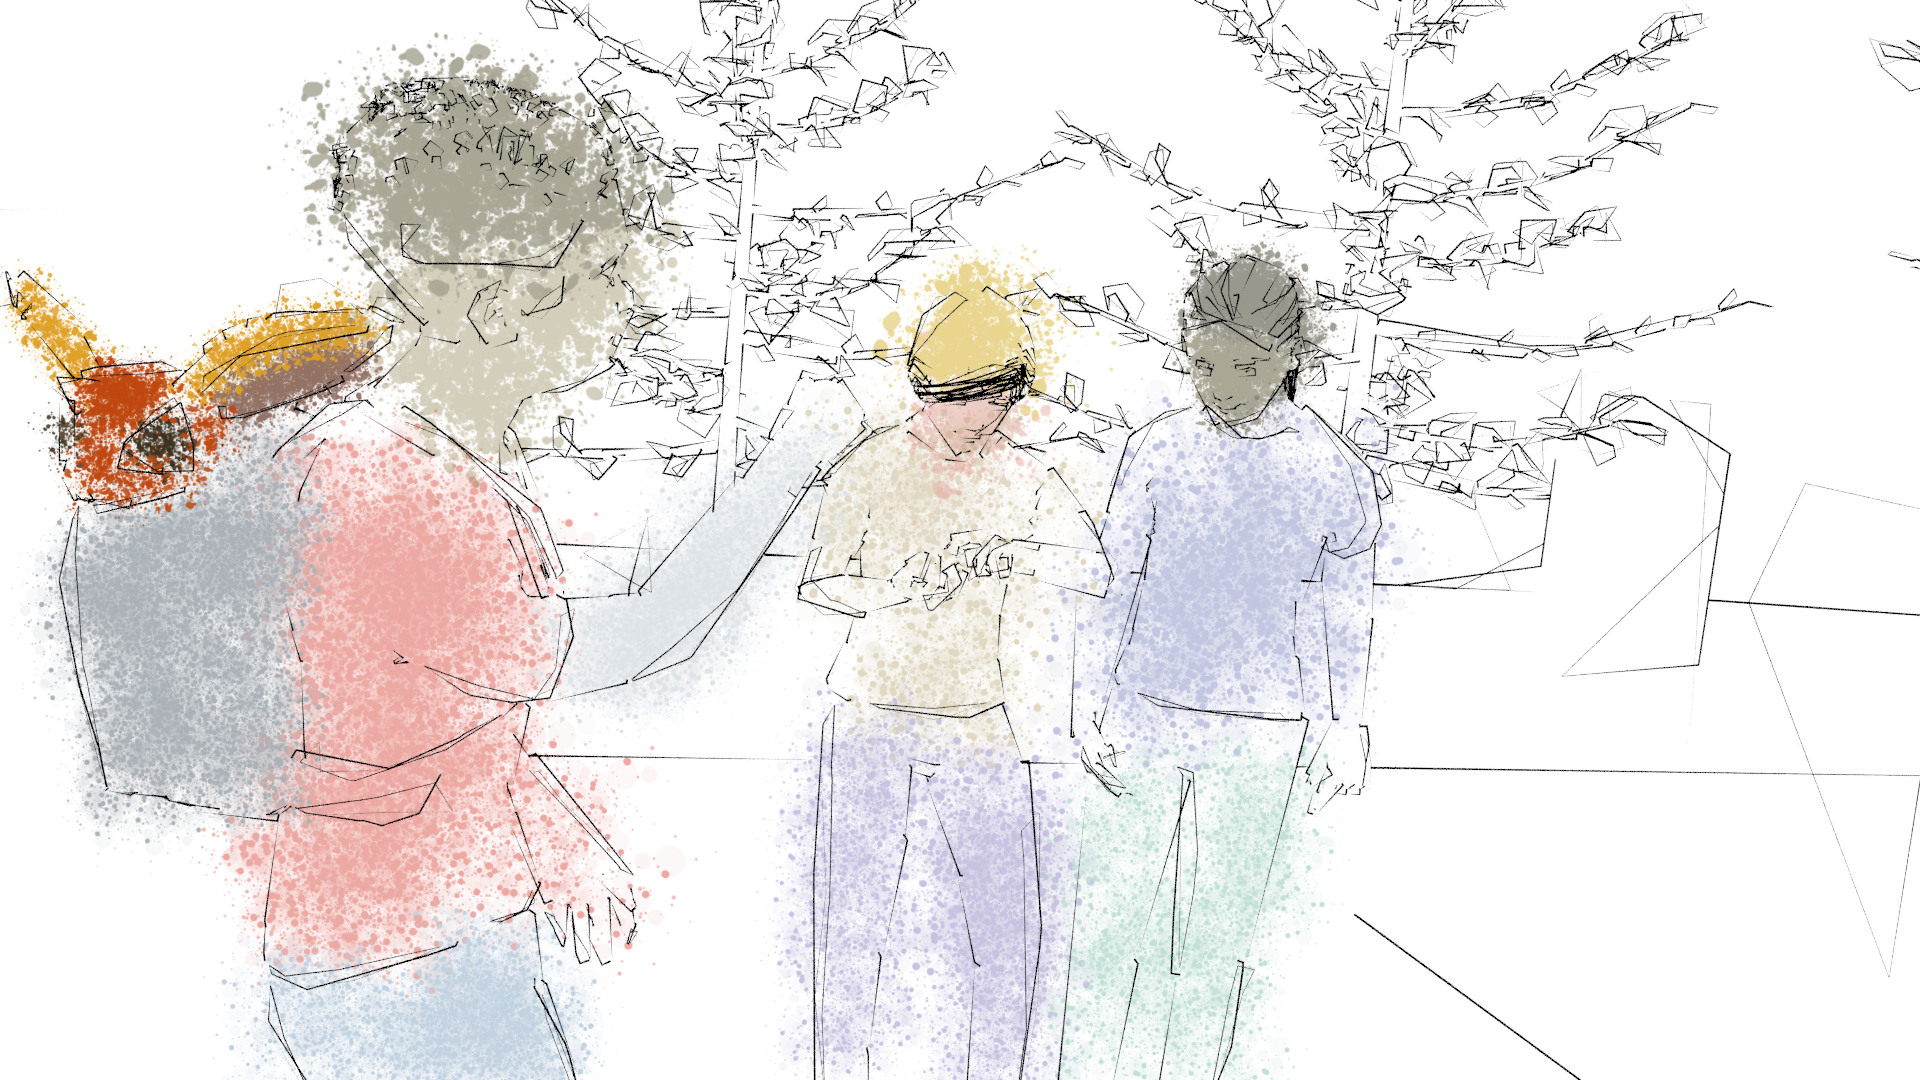
\includegraphics[width=0.9\linewidth]{figs/render5-colors.png}
\end{figure}

\project is a project that aims at helping to build strong human
relationships with the help of technology.

The core idea of the project is to build small companion robots whose
aim is to facilitate human-human interactions. We want to develop these
robots with a particular application in mind: supporting the social and
cultural integration of vulnerable children in a foreign country, and in
particular, migrant children who might lack the otherwise needed support
(shared culture; already well integrated relatives) for a successful
integration.

\subsubsection{Key scientific research questions}

\begin{enumerate}
\item research the role of social influence to scaffold positive human-human
    interactions (including its ethical ramifications) in the context of migrant
    integration;
\item explore how a small robot companion can be endowed with social
    competencies to positively influence human interactions; design and
    implement the corresponding artificial social behaviours;
\item design and build a small rugged and autonomous companion robot that
    realise this goal for child-child interactions; test the technology in
    school with actual migrant children.
\end{enumerate}

\subsubsection{Vision of a novel form of interaction ``human-(robot)-human''}

\paragraph{The case of the social integration of migrant children}

A robot is left with the child when he or she starts their journey in
their new host country, and becomes a companion for the child during the
first months of the integration. Using several mechanisms that are
discussed in this proposal, the robot helps the child to gain
self-confidence, and ultimately engage in successful social interactions
with other children.

Critically, the robot is designed to support the social and cultural
integration of the child \emph{amongst her/his peers}. While the child
might build affective/emotional bonds with the robot over the course of
the support period, the robot behaviour is designed to ensure that these
bonds do not substitute themselves to the interactions with other
children.

The project combines a range of scientific and engineering endeavours to
realise within a 5-years timeframe an ambitious and bold vision for
social robotics in our society. Specifically, the project draws from the
fields of social robotics; human-robot interaction; human-machine
interaction design; and mechatronics.

While the breadth of the proposed project is significant (from
mechatronic design to long-term field testing with vulnerable
populations), the project structure minimizes the cross-dependencies
within the project, avoiding critical failure points that would put the
whole project at risk, and a careful risk assessment is conducted that
includes meaningful mitigation strategies.




\subsection{A principled architecture for socially intelligent robots}


\begin{itemize}
    \item Intrinsic social motivation: do good
    \item bottom-up grounding for situation assessment and social situation
        assessment
    \item symbolic grounding of both environment and social situation using
        'human in the loop' OR data-driven symbolic grounding
    \item knowledge representation and symbolic reasoning for dialogue
        grounding, goal planning, knowledge exchange and linked data
    \item action execution using human-in-the-loop ML
\end{itemize}


\subsection{Cross-disciplinary team, research methodology, and research
infrastructure}

The project's ambitious scientific and technical goals are expected to deliver
major scientific, societal and technical impact, that extends beyond the
boundaries of the fellowship. While ambitious, the project's feasibility is
ensured through a strong combination of cross-disciplinary expertise and
support from the host's unique research infrastructure. Scaffolded by a
participatory and iterative research methodology, and the PI experience in
managing teams and complex projects through his recognised leadership, \project
is set to deliver.

\project is indeed an interdisciplinary endeavour, and requires several
complementary expertises to be successfull. I have assembled a strong and
diverse team, with exceptional expertise both on working with vulnerable refugee
populations, and on designing social robots. The team comprises of institutional
partners with strong expertise in supporting asylum seeker (UK Refugee Council
and [Katheryn Cronin - lawyer]), charities with extensive experience using art
to support refugee populations (ArtRefuge UK), an interaction designer working
on memory collection and recollection with vulnerable children, and several
close academic collaboration: with Dave Meckin (University of the West of
England), senior researcher in media tecnologies with a unique expertise working
with vulnerable children; with Jérémy Bonvoisin (University of Bath), senior
research on sustainable and open hardware development; and finally with Katie
Winkle (University of Bristol/University of the West of England), junior
scientist with a unique expertise in social robotics.

To mirror the cross-disciplinary team, the research methodology developped for
\project will rely heavily on \emph{mutual shaping}, through co-design and
participatory design, and multi-disciplinary development sprints.

\subsubsection{Technical infrastructure}

The \project project sets an ambitious target in term of technical development.
The project indeed requires unique technical skills, both software and
hardware-wise, to create, design and build the envisonned robotic systems.

Software-wise, Dr Lemaignan, the principal investigator, is a leading
developer of software for intelligent robots, with numerous contributions to
the major software platforms used in robotic (including major contributions to
ROS, OpenCV, authoring of widely-used pieces of software like the ROS-naoqi
bridge used by hundred of researchers using the Nao and Pepper robots or the
MORSE robotic simulator). He has been teaching various modules related to
software development for robotics, and the breadth and depth of his knowledge of
robotic software development is well established. He will be leading the
software development, and, as part of the fellowship, he will also seek for
additional expert knowledge on (1) interaction design and (2) low-level
micro-programming to complete the set of required programming needs.

Hardware-wise, the Bristol Robotics Lab, where this fellowship will take place,
offer unique support and facilities for robotic hardware development: the
laboratory's dedicated equipment includes two industrial-grade rapid prototyping
machine, a laser cutter, one 5-axis digital milling machine, all the required
facilities for PCB prototyping, and a team of six full-time technicians,
specialised in hardware development. The BRL has indeed a long track-record of
designing and building new and original robots (from the BERT humanoid in the
FP7 CHRIS project, to micro-robotics [in...?], to [...]). \project will directly
benefit of this expertise, which will ensure a feasible and realistic technical
implementation of the \project robots. Besides, an hardware engineer, dedicated
to the project, will be recruited in the frame of the project.

The BRL also include a hardware incubator and is co-located with 70 start-ups
and SMEs specialising in robotic hardware and mechatronics (Bristol's
\emph{FutureSpace}). This combination of excellent research and vast industry
expertise on one site is unique in the UK, and is will play an instrumental role
in providing a coherent and strong pathway to impact to the project, including
further engagement with industrial partners and spin-off opportunities.








%%%%%%%%%%%%%%%%%%%%%%%%%%%%%%%%%%%%%%%%%%%%%%%%%%%%%%%%%%%%%%%%%%%%%%%%%%%%%
%%%%%%%%%%%%%%%%%%%%%%%%%%%%%%%%%%%%%%%%%%%%%%%%%%%%%%%%%%%%%%%%%%%%%%%%%%%%%
%%%%%%%%%%%%%%%%%%%%%%%%%%%%%%%%%%%%%%%%%%%%%%%%%%%%%%%%%%%%%%%%%%%%%%%%%%%%%

\newpage

\section{B1.b The principal Investigator}\label{the-principal-investigator}

\hypertarget{curriculum-vitae}{%
\subsection{Curriculum vitae}\label{curriculum-vitae}}

\eu{(max 2 pages)}

%%%%%%%%%%%%%%%%%%%%%%%%%%%%%%%%%%%%%%%%%%%%%%%%%%%%%%%%%%%%%%%%%%%%%%%%%%%%%
%%%%%%%%%%%%%%%%%%%%%%%%%%%%%%%%%%%%%%%%%%%%%%%%%%%%%%%%%%%%%%%%%%%%%%%%%%%%%
%%%%%%%%%%%%%%%%%%%%%%%%%%%%%%%%%%%%%%%%%%%%%%%%%%%%%%%%%%%%%%%%%%%%%%%%%%%%%
\newpage
\subsection{B1.2 Early achievements track-record}\label{early-achievements-track-record}

\eu{(max 2 pages)}

Dr Séverin Lemaignan is Senior Researcher at the Bristol Robotics
Laboratory, University of the West of England, Bristol. Previously, he
obtained a joint PhD in Cognitive Robotics from the CNRS/LAAS (France)
and the Technical University of Munich (Germany) for which he received
the Best PhD in Robotics 2012 award from French CNRS. He then conducted
his research as Research Fellow at EPFL (Switzerland) and Plymouth
University (UK) where he was Lecturer in Robotics until 2018. Dr Séverin
Lemaignan has been involved in several European projects related to
social and cognitive robotics: CHRIS (Cooperative Human Robot
Interaction Systems), DREAM (Development of Robot-Enhanced therapy for
children with AutisM spectrum disorders), L2TOR (Second language
TutOring using social Robots). He has also been awarded in 2015 a EU
H2020 Marie Sklodowska-Curie Individual Fellowship for his project
DoRoThy (Donating Robots a Theory of Mind). His research interests
primarily concern the socio-cognitive aspects of human-robot
interaction, both from the perspective of the human cognition and the
design of cognitive architectures for the robots. More recently, he has
been focusing his experimental work on child-robot interactions in
educative settings, exploring how robots can support teachers and
therapists to develop effective and engaging novel learning paradigms.
















%%%%%%%%%%%%%%%%%%%%%%%%%%%%%%%%%%%%%%%%%%%%%%%%%%%%%%%%%%%%%%%%%%%%%%%%%%%%%
%%%%%%%%%%%%%%%%%%%%%%%%%%%%%%%%%%%%%%%%%%%%%%%%%%%%%%%%%%%%%%%%%%%%%%%%%%%%%
%%%%%%%%%%%%%%%%%%%%%%%%%%%%%%%%%%%%%%%%%%%%%%%%%%%%%%%%%%%%%%%%%%%%%%%%%%%%%
\newpage

\section{B2. The scientific proposal}\label{part-b2-the-scientific-proposal}

\eu{(max 15 pages)}

\hypertarget{a.-state-of-the-art-and-objectives}{%
\subsection{a. State of the art and
objectives}\label{a.-state-of-the-art-and-objectives}}

\hypertarget{b.-methodology}{%
\subsection{b. Methodology}\label{b.-methodology}}

\subsection{Novelty, non-incrementality, plausibility and foundational character}

\subsubsection{Companion robots}

One example of a small, rugged robot designed for intensive use in school
environments is Cellulo~\footcite{ozgur2017cellulo}.

\begin{figure}[!htbp]
    \begin{minipage}[b]{.3\linewidth}
        \centering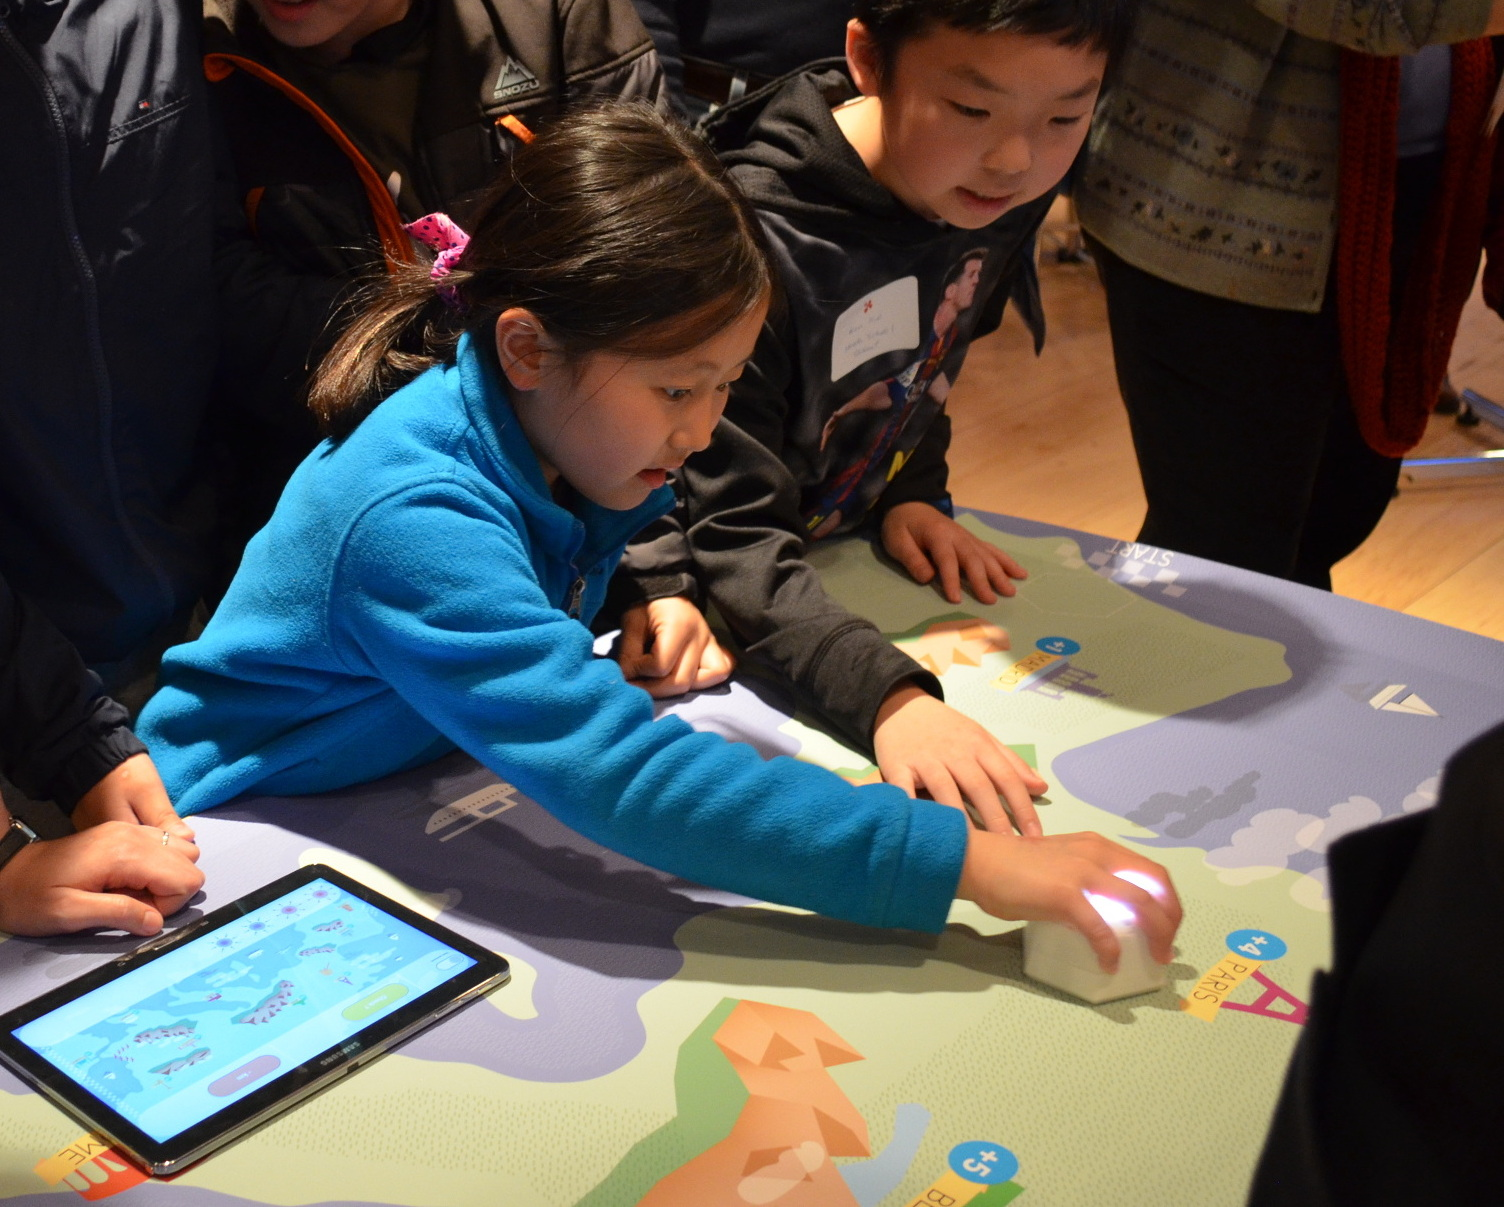
\includegraphics[height=4cm]{figs/cellulo.jpg}
        \subcaption{EPFL's Cellulo robot}\label{fig:cellulo}
    \end{minipage}%
    \hspace{0.5cm}
    \begin{minipage}[b]{.3\linewidth}
        \centering
        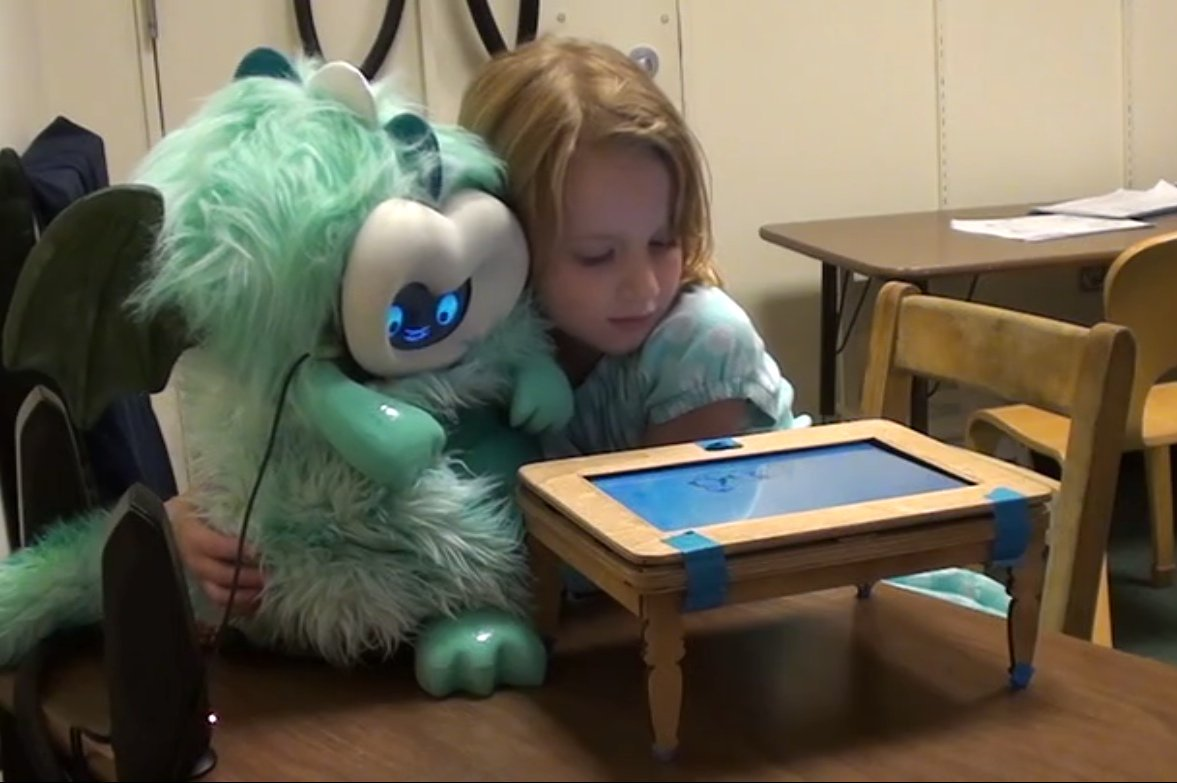
\includegraphics[height=4cm]{figs/tega.jpg}
        \subcaption{MediaLab's Tega robot}\label{fig:tega}
    \end{minipage}
    \hspace{0.5cm}
    \begin{minipage}[b]{.3\linewidth}
        \centering
        %\includegraphics[height=4cm]{figs/ono.png}
        \subcaption{OPSORO's Ono robot}\label{fig:ono}
    \end{minipage}
    \caption{Existing research-level companion robots}\label{fig:research-robots}
\end{figure}

\begin{figure}[!htbp]
    \begin{minipage}[b]{.3\linewidth}
        \centering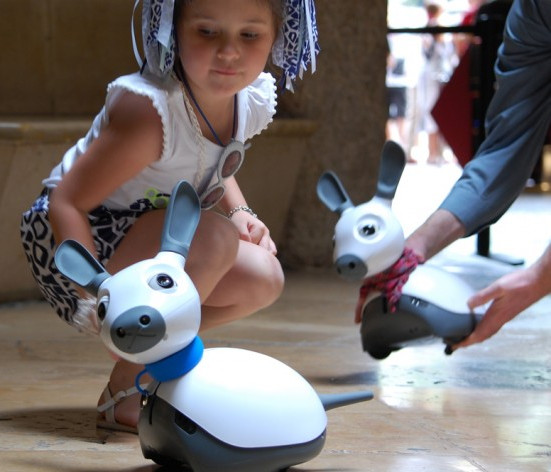
\includegraphics[height=4cm]{figs/miro.jpg}
        \subcaption{Consequential's Miro robot}\label{fig:miro}
    \end{minipage}%
    \hspace{0.1cm}
    \begin{minipage}[b]{.3\linewidth}
        \centering
        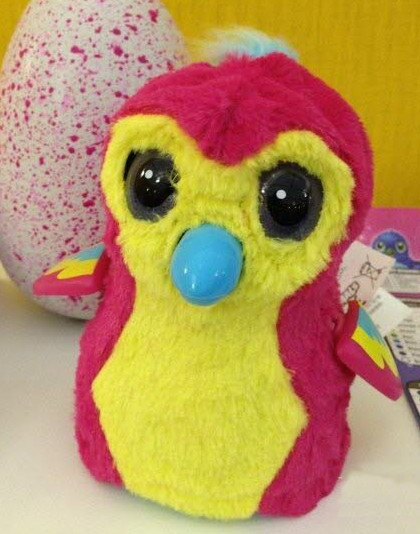
\includegraphics[height=4cm]{figs/hatchnimals.jpg}
        \subcaption{SpinMaster's Hatchimals}\label{fig:hatchimals}
    \end{minipage}%
    \hspace{0.1cm}
    \begin{minipage}[b]{.3\linewidth}
        \centering
        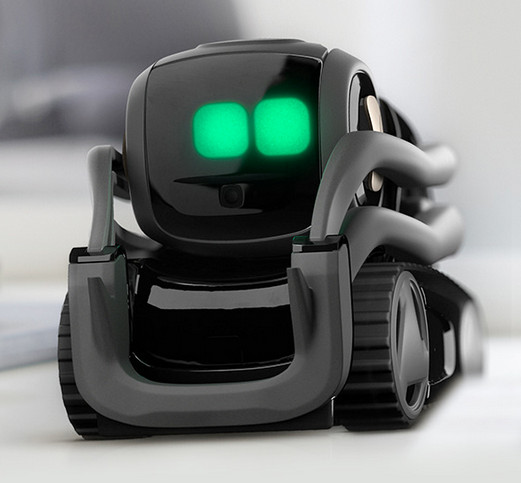
\includegraphics[height=4cm]{figs/anki-vector.jpg}
        \subcaption{Anki's Vector}\label{fig:vector}
    \end{minipage}
    \caption{Existing commercial companion robots}\label{fig:commercial-robots}
\end{figure}

\subsubsection{Social influence}

\begin{figure}[!htbp]
\centering
    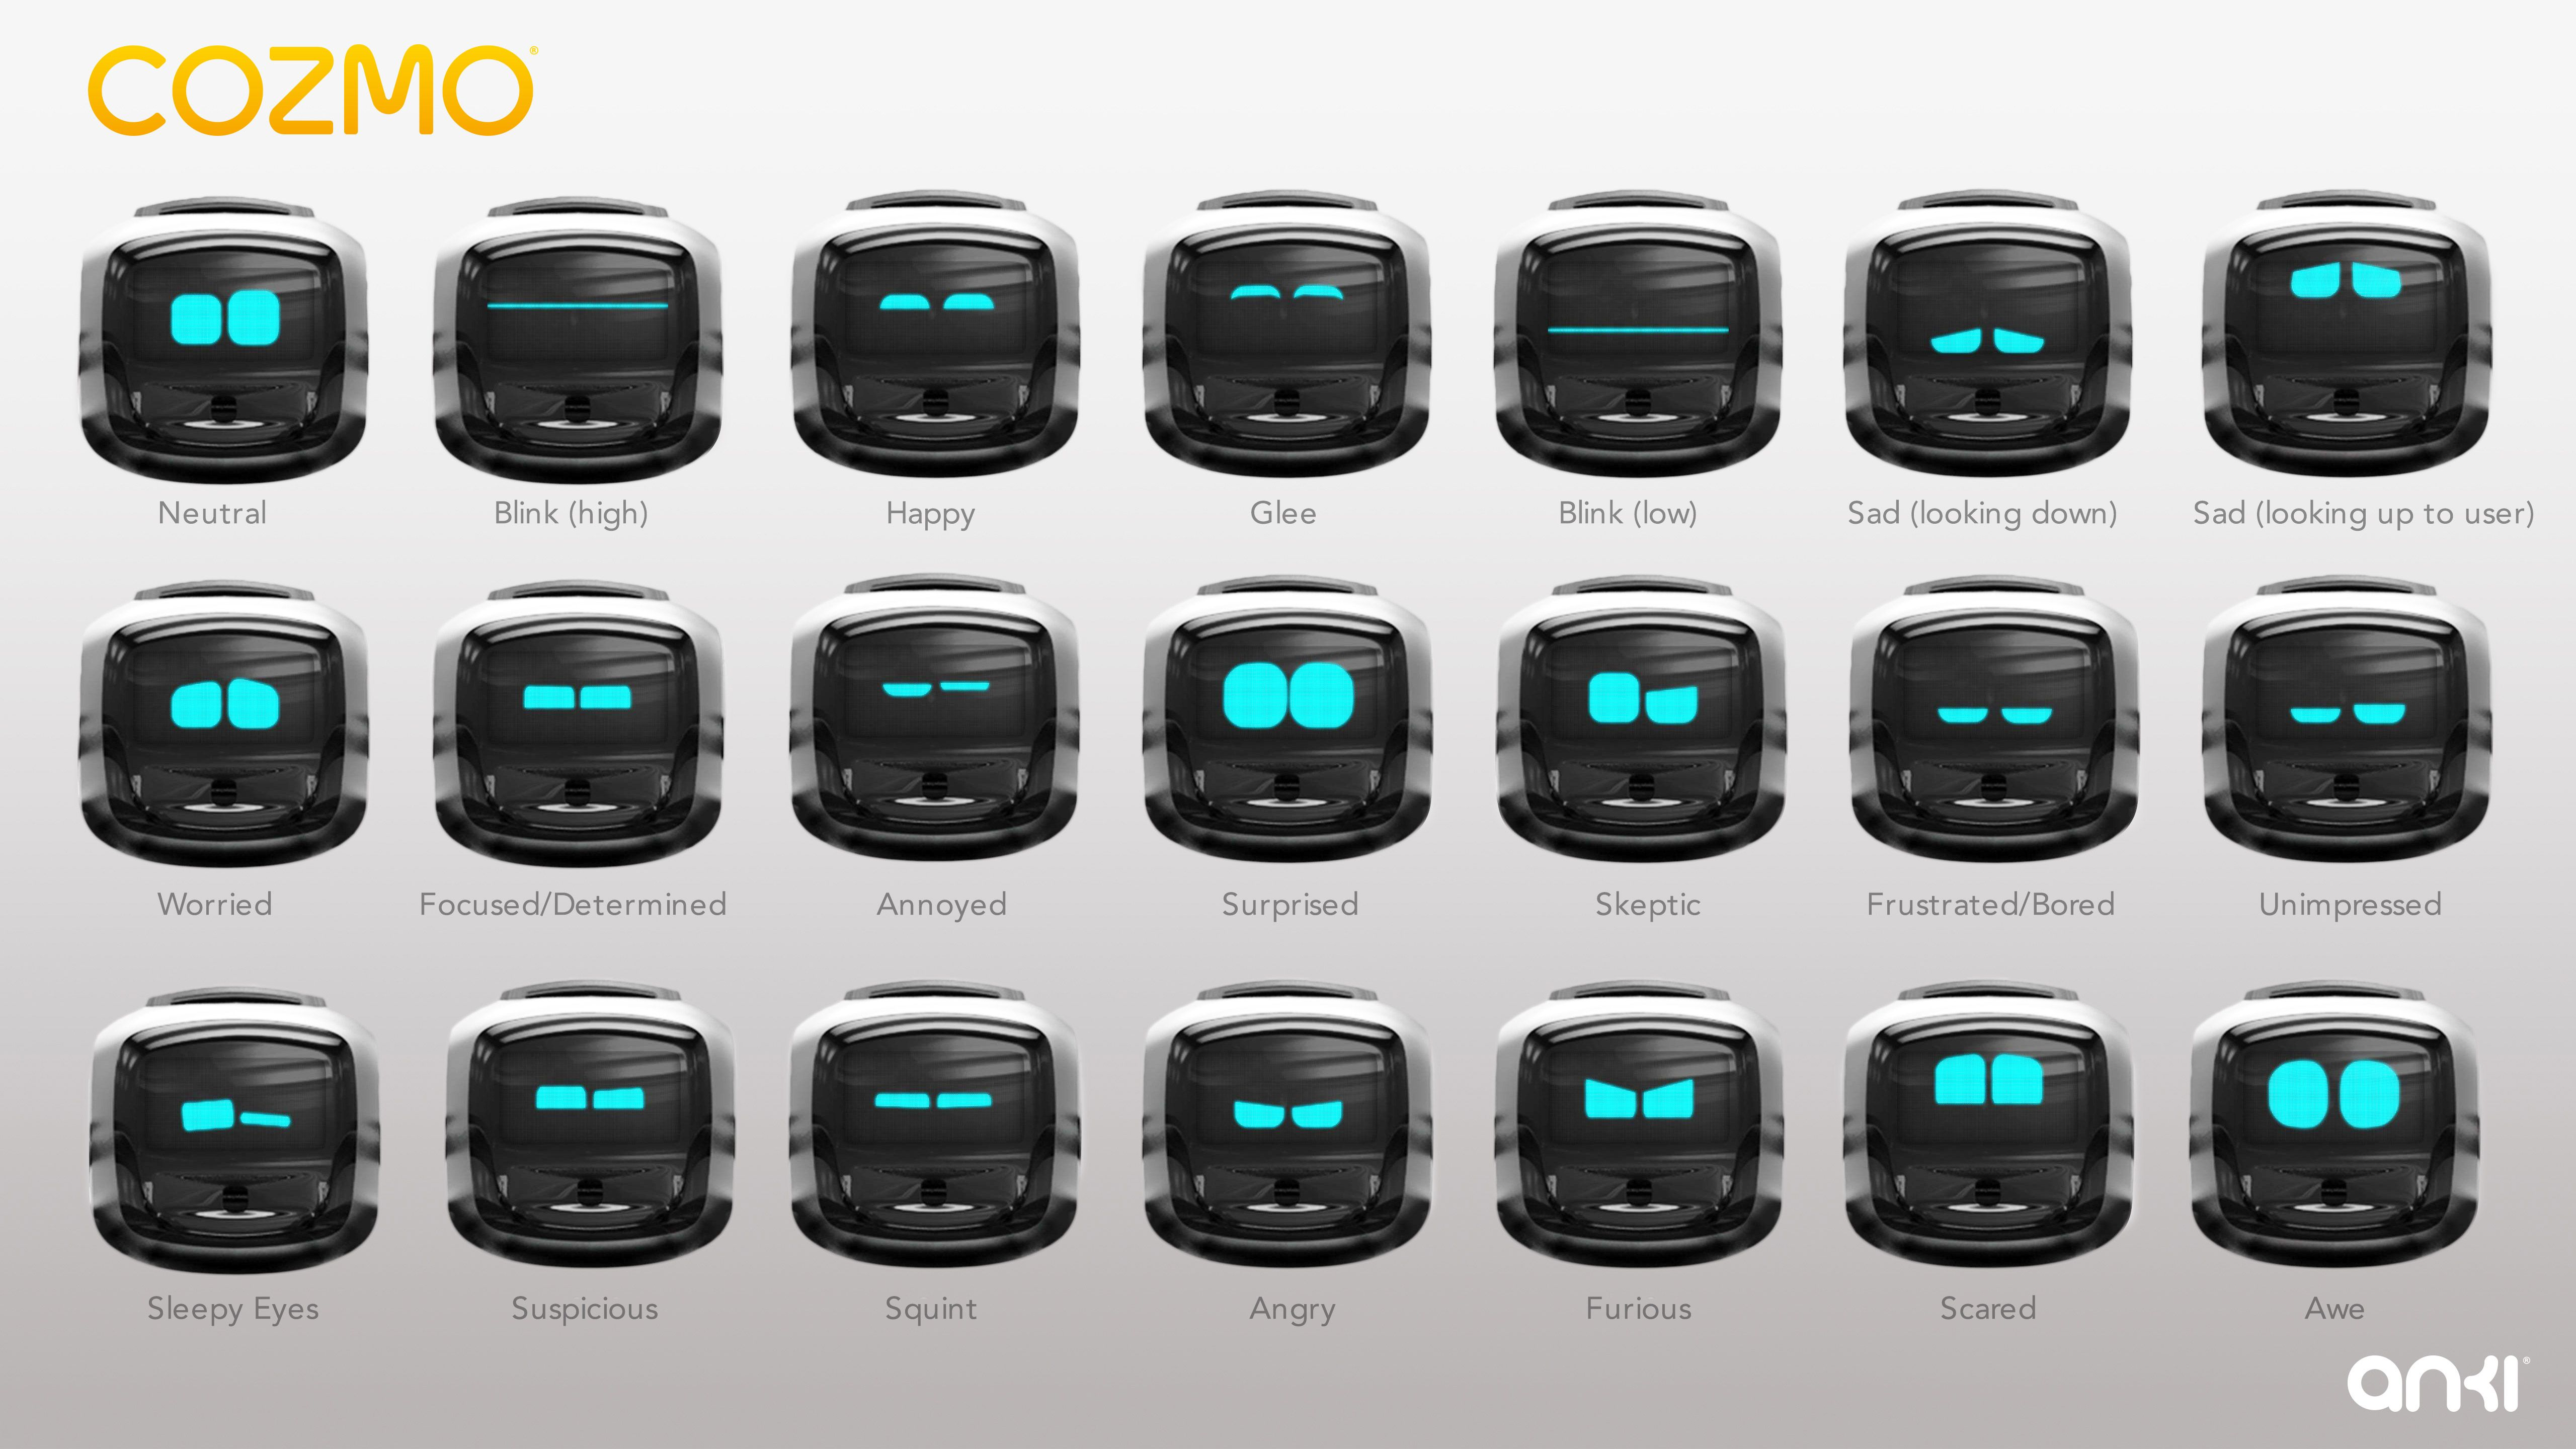
\includegraphics[width=0.7\textwidth]{figs/cozmo-expression-sheet.jpg}
\caption{Cozmo facial expressions}
\end{figure}


\subsection{Research methodology}\label{research-methodology}


\subsubsection{Deployments in schools}

\subsection{Interdisciplinarity}
%%%%%%%%%%%%%%%%%%%%%%%%%%%%%%%%%%%%%%%%%%%%%%%%%%%%%%%%%%%%%%%%%%%%%%%%%%%%%%%%%%%%%%%%
%%%%%%%%%%%%%%%%%%%%%%%%%%%%%%%%%%%%%%%%%%%%%%%%%%%%%%%%%%%%%%%%%%%%%%%%%%%%%%%%%%%%%%%%
%%%%%%%%%%%%%%%%%%%%%%%%%%%%%%%%%%%%%%%%%%%%%%%%%%%%%%%%%%%%%%%%%%%%%%%%%%%%%%%%%%%%%%%%

\newpage
\section{Impact}\label{impact}

\subsection{Impact on society and technology: building an inclusive society}

\subsection{Impact on future leadership}

\subsection{Measures for achieving impact}

\subsubsection{Dissemination and exploitation of results}

\subsubsection{Communication activities}


%%%%%%%%%%%%%%%%%%%%%%%%%%%%%%%%%%%%%%%%%%%%%%%%%%%%%%%%%%%%%%%%%%%%%%%%%%%%%%%%%%%%%%%%
%%%%%%%%%%%%%%%%%%%%%%%%%%%%%%%%%%%%%%%%%%%%%%%%%%%%%%%%%%%%%%%%%%%%%%%%%%%%%%%%%%%%%%%%
%%%%%%%%%%%%%%%%%%%%%%%%%%%%%%%%%%%%%%%%%%%%%%%%%%%%%%%%%%%%%%%%%%%%%%%%%%%%%%%%%%%%%%%%
\newpage
\section{Implementation}\label{part3}

%%%%%%%%%%%%%%%%%%%%%%%%%%%%%%%%%%%%%%%%%%%%%%%%%%%%%%%%%%%%%%%%%%%%%%%%%%%%%%%%%%%%%%%
%% Names of the Work packages

\newcommand{\wpOne}{Project management}
\newcommand{\wpOneShort}{\wpOne{}}

\newcommand{\wpTwo}{Technology to socially influence human-human interactions}
\newcommand{\wpTwoShort}{Social influence}


\newcommand{\wpThree}{Interaction design for robot-supported human-human interactions}
\newcommand{\wpThreeShort}{Interaction design}

\newcommand{\wpFour}{Design and building of a companion robot for social interaction in the field}
\newcommand{\wpFourShort}{Companion robot creation}

\newcommand{\wpFive}{AI for social cognition}
\newcommand{\wpFiveShort}{AI for social cognition}

\newcommand{\wpSix}{Dissemination and exploitation}
\newcommand{\wpSixShort}{Dissemination}


%%%%%%%%%%%%%%%%%%%%%%%%%%%%%%%%%%%%%%%%%%%%%%%%%%%%%%%%%%%%%%%%%%%%%%%%%%%%%%%%%%%%%%%


\subsection{Workplan and intermediate targets}

\subsubsection{Project structure}

\begin{table}[!htbp]
    \begin{tabular}{@{}p{1cm}p{6cm}p{2cm}p{2cm}p{1.5cm}p{1.5cm}p{1.5cm}@{}}
\toprule
\textbf{WP} & \textbf{Work package title} & \textbf{Lead participant No} & \textbf{Lead participant short name} & \textbf{Person-Months} & \textbf{Start month} & \textbf{End month} \\ \midrule
1                        & \wpOne                      &                              &                                      &                        &                      &                    \\
2                        & \wpTwo                      &                              &                                      &                        &                      &                    \\
3                        & \wpThree                    &                              &                                      &                        &                      &                    \\
4                        & \wpFour                     &                              &                                      &                        &                      &                    \\
5                        & \wpFive                     &                              &                                      &                        &                      &                    \\
6                        & \wpSix                      &                              &                                      &                        &                      &                    \\
                         &                             &                              &                                      & \textbf{Total months}  &                      &                    \\ \bottomrule
\end{tabular}
\end{table}


\subsubsection{Work package 1: \wpOne}

\begin{table}[!htbp]
\centering
\begin{tabular}{|l|p{1.5cm}|p{1.5cm}|p{1.5cm}|p{1.5cm}|p{1.5cm}|p{1.5cm}|p{1.5cm}|}
\hline
Work package number            & 1 & \multicolumn{3}{l|}{Lead beneficiary} & \multicolumn{3}{l|}{\bf BRL} \\ \hline
Work package title             & \multicolumn{7}{l|}{\wpOne}                                             \\ \hline
Participant number             &     &         &         &                  &       &       &      \\ \hline
Short name of participant      &     &         &         &                  &       &       &      \\ \hline
Person/months per participant: &     &         &         &                  &       &       &      \\ \hline
Start month                    & \multicolumn{3}{l|}{}  & End month        & \multicolumn{3}{l|}{} \\ \hline
\end{tabular}
\end{table}


\textbf{Objectives:}

\textbf{Description of work:}

\ldots{}description\ldots{}

\task{1.1}{}

\vspace{0.5cm}\textbf{Deliverables:}

\begin{itemize}

\item   \emph{Deliverable D1.1} (Month 2): website and logo
\end{itemize}

\subsubsection{Work package 2: \wpTwo}

\begin{table}[!htbp]
\centering
\begin{tabular}{|l|p{1.5cm}|p{1.5cm}|p{1.5cm}|p{1.5cm}|p{1.5cm}|p{1.5cm}|p{1.5cm}|}
\hline
Work package number            & 2 & \multicolumn{3}{l|}{Lead beneficiary} & \multicolumn{3}{l|}{} \\ \hline
Work package title             & \multicolumn{7}{l|}{\wpTwo}                                       \\ \hline
Participant number             &     &         &         &                  &       &       &      \\ \hline
Short name of participant      &     &         &         &                  &       &       &      \\ \hline
Person/months per participant: &     &         &         &                  &       &       &      \\ \hline
Start month                    & \multicolumn{3}{l|}{}  & End month        & \multicolumn{3}{l|}{} \\ \hline
\end{tabular}
\end{table}

\textbf{Objectives:}
\textbf{Description of work:}

\ldots{}description\ldots{}

\task{2.1}{Identification of the dimensions of social influence for human interpersonal interactions}

\task{2.2}{Ethics of social influence}
Blah blah

\task{2.3}{Study 1 -- Socially influencing companion robot}
First study, using Anki's Vector robot.

\vspace{0.5cm}\textbf{Deliverables:}

\begin{itemize}
    \item \D{2.1}{12}{great report}
\end{itemize}

\subsubsection{Work package 3: \wpThree}

\begin{table}[!htbp]
\centering
\begin{tabular}{|l|p{1.5cm}|p{1.5cm}|p{1.5cm}|p{1.5cm}|p{1.5cm}|p{1.5cm}|p{1.5cm}|}
\hline
Work package number            & 3 & \multicolumn{3}{l|}{Lead beneficiary} & \multicolumn{3}{l|}{} \\ \hline
Work package title             & \multicolumn{7}{l|}{\wpThree}                                     \\ \hline
Participant number             &     &         &         &                  &       &       &      \\ \hline
Short name of participant      &     &         &         &                  &       &       &      \\ \hline
Person/months per participant: &     &         &         &                  &       &       &      \\ \hline
Start month                    & \multicolumn{3}{l|}{}  & End month        & \multicolumn{3}{l|}{} \\ \hline
\end{tabular}
\end{table}

\textbf{Objectives:}

\begin{itemize}
    \item refine interaction modalities (in
    particular, the non-verbal speech), details cross-modal interactions,
    define interaction patterns with the child
\end{itemize}

\ldots{}description\ldots{}

\task{3.1}{Analysis of needs}
\task{3.2}{Cross-cultural interactions}

\vspace{0.5cm}\textbf{Deliverables:}

\begin{itemize}
    \item \D{3.1}{12}{great report}
\end{itemize}

\subsubsection{Work package 4: \wpFour}

\begin{table}[!htbp]
\centering
\begin{tabular}{|l|p{1.5cm}|p{1.5cm}|p{1.5cm}|p{1.5cm}|p{1.5cm}|p{1.5cm}|p{1.5cm}|}
\hline
Work package number            & 4 & \multicolumn{3}{l|}{Lead beneficiary} & \multicolumn{3}{l|}{} \\ \hline
Work package title             & \multicolumn{7}{l|}{\wpFour}                                      \\ \hline
Participant number             &     &         &         &                  &       &       &      \\ \hline
Short name of participant      &     &         &         &                  &       &       &      \\ \hline
Person/months per participant: &     &         &         &                  &       &       &      \\ \hline
Start month                    & \multicolumn{3}{l|}{}  & End month        & \multicolumn{3}{l|}{} \\ \hline
\end{tabular}
\end{table}


\begin{itemize}
    \item long term interaction
    \item one full day of autonomy
    \item rugged \footcite{ozgur2017cellulo, hostettler2016realtime}
    \item child friendly: mechanical constraints~\footcite{ozgur2016permanent} + design
\end{itemize}


\textbf{Description of work:}

Develop a novel platform, including:

\begin{itemize}
    \item chassis
    \item power autonomy for one day
    \item on-board compute suitable for deep learning (NVidia Xavier?)
    \item vision (embedded RGB-D camera)
    \item audio processing
\end{itemize}

\ldots{}

\task{4.1}{Physical design of the robot companion}
\task{4.2}{Interaction design}
\task{4.3}{Mechatronics \& Sensing}
\task{4.4}{On-board data processing}
\task{4.5}{System integration}

\begin{itemize}
    \item \D{4.1}{12}{great report}
\end{itemize}

\subsubsection{Work package 5: \wpFive}

\begin{table}[!htbp]
\centering
\begin{tabular}{|l|p{1.5cm}|p{1.5cm}|p{1.5cm}|p{1.5cm}|p{1.5cm}|p{1.5cm}|p{1.5cm}|}
\hline
Work package number            & 5 & \multicolumn{3}{l|}{Lead beneficiary} & \multicolumn{3}{l|}{} \\ \hline
Work package title             & \multicolumn{7}{l|}{\wpFive}                                      \\ \hline
Participant number             &     &         &         &                  &       &       &      \\ \hline
Short name of participant      &     &         &         &                  &       &       &      \\ \hline
Person/months per participant: &     &         &         &                  &       &       &      \\ \hline
Start month                    & \multicolumn{3}{l|}{}  & End month        & \multicolumn{3}{l|}{} \\ \hline
\end{tabular}
\end{table}


\textbf{Objectives:}

\textbf{Description of work:}

\ldots{}description\ldots{}

\task{5.1}{Multi-modal communication}
\task{5.2}{Social awareness}
\task{5.3}{Machine learning of social behaviours}
\task{5.4}{Social controller}

\vspace{0.5cm}\textbf{Deliverables:}

\begin{itemize}
    \item \D{5.1}{12}{great report}
\end{itemize}

\subsubsection{Work package 6: \wpSix}

\begin{table}[!htbp]
\centering
\begin{tabular}{|l|p{1.5cm}|p{1.5cm}|p{1.5cm}|p{1.5cm}|p{1.5cm}|p{1.5cm}|p{1.5cm}|}
\hline
Work package number            & 6 & \multicolumn{3}{l|}{Lead beneficiary} & \multicolumn{3}{l|}{} \\ \hline
Work package title             & \multicolumn{7}{l|}{\wpSix}                                       \\ \hline
Participant number             &     &         &         &                  &       &       &      \\ \hline
Short name of participant      &     &         &         &                  &       &       &      \\ \hline
Person/months per participant: &     &         &         &                  &       &       &      \\ \hline
Start month                    & \multicolumn{3}{l|}{}  & End month        & \multicolumn{3}{l|}{} \\ \hline
\end{tabular}
\end{table}


\textbf{Objectives:}

\textbf{Description of work:}

\ldots{}description\ldots{}

\task{6.1}{Academic dissemination}
\task{6.2}{General public dissemination}
\task{6.3}{Commercial exploitation}

\vspace{0.5cm}\textbf{Deliverables:}

\begin{itemize}
    \item \D{6.1}{12}{website and logo}
\end{itemize}

\subsubsection{Deliverables overview}\label{deliverables-overview}

\begin{table}[!htbp]
\caption{List of deliverables}
\begin{tabular}{@{}lllllll@{}}
\toprule
\textbf{Deliverable} & \textbf{Deliverable name} & \textbf{Work package No} & \textbf{Lead participant short name} & \textbf{Type} & \textbf{Dissemination level} & \textbf{Delivery date} \\ \midrule
D1.1                 &                           &                          &                                      &               &                              &                        \\
D1.2                 &                           &                          &                                      &               &                              &                        \\
D2.1                 &                           &                          &                                      &               &                              &                        \\
...                  &                           &                          &                                      &               &                              &                        \\ \bottomrule
\end{tabular}
\end{table}

Type:

\begin{itemize}

\item   R: Document, report (excluding the periodic and final reports)
\item   DEM: Demonstrator, pilot, prototype, plan designs
\item   DEC: Websites, patents filing, press \& media actions, videos, etc.
\item   OTHER: Software, technical diagram, etc.
\end{itemize}

Dissemination level:

\begin{itemize}

\item   PU = Public, fully open, e.g.~web
\item   CO = Confidential, restricted under conditions set out in Model Grant
  Agreement
\item   CI = Classified, information as referred to in Commission Decision
  2001/844/EC.
\end{itemize}

\subsubsection{Gantt chart}\label{gantt-chart}

\begin{landscape}
%%%%%%%%%%%%%%%%%
%%
%% Task dependencies
%%
%% Task...        depends on Task...
%% T1.3           T1.1
%% T1.3           T1.2
%% T1.2           T2.2 (user interface)
%% T3.3           T2.3
%%

\definecolor{barcolor}{RGB}{153,204,254}
\definecolor{linkred}{RGB}{165,0,33}
%\renewcommand\sfdefault{phv}
%\renewcommand\mddefault{mc}
%\renewcommand\bfdefault{bc}
\setganttlinklabel{s-s}{START-TO-START}
\setganttlinklabel{f-s}{}
\setganttlinklabel{f-f}{FINISH-TO-FINISH}

%\begin{sidewaysfigure}[!ht]
\begin{figure}[!ht]

%\sffamily
\begin{ganttchart}[
        canvas/.append style={fill=none, draw=black!5, line width=.75pt},
        hgrid style/.style={draw=black!5, line width=.75pt},
        vgrid={*1{draw=black!5, line width=.75pt}},
        %vgrid={*1{black}, *{11}{black!5}}, % doesnt work for some reason
        x unit=.35cm,
        y unit chart=.65cm,
        time slot format=isodate-yearmonth,
        time slot unit=month, % pgfgantt >= 5.0
        %compress calendar, % pgfgantt < 5.0 => overleaf
        title/.style={draw=none, fill=none},
        title label font=\bfseries\footnotesize,
        %title label node/.append style={below=7pt},
        include title in canvas=false,
        bar label font=\mdseries\small\color{black!70},
        %bar label node/.append style={left=2cm},
        bar/.append style={draw=none, fill=barcolor!50},
        bar progress label font=\mdseries\footnotesize\color{black!70},
        group/.append style={fill=barcolor},
        group incomplete/.append style={fill=black},
        group left shift=0,
        group right shift=0,
        group height=.5,
        group peaks tip position=0,
        group label node/.append style={left=.6cm},
        group progress label font=\bfseries\small,
        link/.style={-latex, line width=1.5pt, linkred},
        link label font=\scriptsize\bfseries,
        link label node/.append style={below left=-2pt and 0pt,
        milestone/.append style={circle},
        milestone inline label node/.append style={left=5mm}}
    ]{2021-01}{2025-12}
    
        %\gantttitle[
        %    title label node/.append style={below left=7pt and -3pt}
        %]{Month:\quad1}{1}
        \gantttitlecalendar{year, month} \\
        %\gantttitlelist{0,5,...,60}{1} \\
        %% WP1
        \ganttgroup[]{WP1 \wpOneShort}{2021-01}{2023-12} \\
            \ganttbar[name=WP11]{\textbf{1.1} Conceptual framing \& ethics}{2021-01}{2023-12} \\
            \ganttbar[name=WP12prep,inline,bar/.append style={fill=gray!20}]{preparation}{2021-07}{2021-12}
            \ganttbar[name=WP12exp,inline]{WeTheCurious experiment}{2022-01}{2022-12}
            \ganttbar[name=WP12]{\textbf{1.2} Principles of r-HHI}{2023-01}{2023-06} \\

        %\ganttlink[link type=f-s]{WBS1A}{WBS1B}

        %% WP2
        \definecolor{barcolor}{RGB}{153,2,254}
        \ganttgroup[]{WP2 \wpTwoShort}{2021-01}{2024-12} \\
            \ganttbar[name=WP21]{\textbf{2.1} Situation assessment}{2021-01}{2022-06} \\
            \ganttbar[name=WP22]{\textbf{2.2} Social dynamics}{2022-01}{2023-12} \\
            \ganttbar[name=WP23]{\textbf{2.3} Group dynamics}{2024-01}{2024-12} \\
            \ganttbar[name=WP24]{\textbf{2.4} Social situation assessment}{2022-07}{2024-12} \\

        %\ganttlink[link type=f-s]{WP21}{WP24}
        %\ganttlink[link type=f-s]{WP22}{WP23}

        %% WP3
        \definecolor{barcolor}{RGB}{50,220,134}
        \ganttgroup[]{WP3 \wpThreeShort}{2021-01}{2025-12} \\
            \ganttbar[name=WP31]{\textbf{3.1} Social teleology}{2023-01}{2024-12} \\
            \ganttbar[name=WP32]{\textbf{3.2} Human-in-the-loop policy learning}{2021-07}{2025-06} \\
            \ganttbar[name=WP33]{\textbf{3.3} Integrated cognitive architecture}{2021-01}{2025-06} \\

        %\ganttlink[link type=f-s]{WP12}{WP32}

        %% WP4
        \definecolor{barcolor}{RGB}{244,50,20}
        \ganttgroup[]{WP4 \wpFourShort}{2022-01}{2025-12} \\
            \ganttbar[name=WP41]{\textbf{4.1} Behaviours baselining}{2022-01}{2022-12} \\
            \ganttbar[name=WP42]{\textbf{4.2} Generative behaviours}{2023-01}{2023-12} \\
            \ganttbar[name=WP43]{\textbf{4.3} Non-verbal behaviours}{2023-07}{2025-12} \\


        %% WP5
        \definecolor{barcolor}{RGB}{234,200,20}
        \ganttgroup[]{WP5 \wpFiveShort}{2022-07}{2025-12} \\
            \ganttbar[name=WP51prep,inline,bar/.append style={fill=gray!20}]{preparation}{2022-07}{2022-12}
            \ganttbar[name=WP51]{\textbf{5.1} SEN schools experiment}{2023-01}{2023-12} 
            \ganttbar[name=WP51expl,inline,bar/.append style={fill=gray!20}]{analysis}{2024-01}{2024-06} \\
            \ganttbar[name=WP52prep,inline,bar/.append style={fill=gray!20}]{preparation}{2024-01}{2024-06}
            \ganttbar[name=WP52]{\textbf{5.2} children hospital experiment}{2024-07}{2025-06}
            \ganttbar[name=WP52expl,inline,bar/.append style={fill=gray!20}]{analysis}{2025-07}{2025-12} \\

        %\ganttlink[link type=f-s]{WP41}{WP51}


        %\ganttlink[link type=f-s]{WBS1B}{WBS1C}
        %\ganttlink[link type=f-f,link label node/.append style=left]{WBS1C}{WBS1D}

        \ganttmilestone{\bf\sc Integration sprints}{2021-06}
        \ganttmilestone[milestone/.append style={fill=orange, circle}]{}{2021-11}
        \ganttmilestone{}{2022-06}
        \ganttmilestone[milestone/.append style={fill=orange, circle}]{}{2022-11}
        \ganttmilestone{}{2023-06}
        \ganttmilestone{}{2023-12}
        \ganttmilestone[milestone/.append style={fill=orange, circle}]{}{2024-05}
        \ganttmilestone{}{2024-12}


        % separate years
        \ganttvrule[vrule/.append style={gray, dotted, thin}]{}{2021-12}
        \ganttvrule[vrule/.append style={gray, dotted, thin}]{}{2022-12}
        \ganttvrule[vrule/.append style={gray, dotted, thin}]{}{2023-12}
        \ganttvrule[vrule/.append style={gray, dotted, thin}]{}{2024-12}


        \ganttvrule{start @WeTheCurious}{2021-12}
        \ganttvrule{start @SEN school}{2022-12}
        \ganttvrule{start @Children hospital}{2024-06}

\end{ganttchart}

%\end{sidewaysfigure}
\end{figure}

\end{landscape}

\subsubsection{Workpackage interrelations}\label{workpackage-interrelations}

\begin{figure}[!htbp]
    \centering
    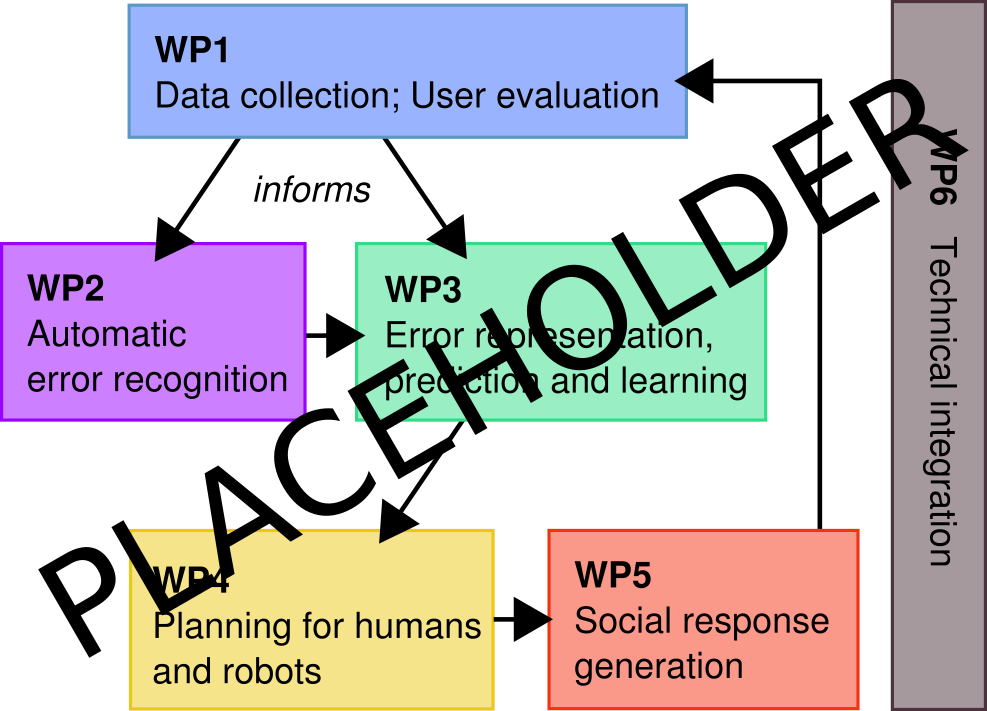
\includegraphics[width=0.8\linewidth]{figs/wp-interrelations}
    \caption{Inter-dependencies between work packages and main tasks}
    \label{}
\end{figure}



\subsection{Management structure, milestones and procedures}\label{management-structure-milestones-and-procedures}

\subsubsection{Milestones}\label{milestones}

\begin{itemize}

\item   week-long tests with local children in local schools
\item   field deployment with one child in one school
\end{itemize}

\begin{table}[!htbp]
\caption{List of milestones}
\centering
\begin{tabular}{@{}lllll@{}}
\toprule
\textbf{Milestone number} & \textbf{Milestone name} & \textbf{Related work package(s)} & \textbf{Estimated date} & \textbf{Means of verification} \\ \midrule
                          &                         &                                  &                         &                                \\
                          &                         &                                  &                         &                                \\
                          &                         &                                  &                         &                                \\
                          &                         &                                  &                         &                                \\ \bottomrule
\end{tabular}
\end{table}


\subsubsection{Risks}\label{risks}

\begin{table}[!htbp]
\caption{Identified risks and proposed mitigations}
\centering
\begin{tabular}{@{}lll@{}}
\toprule
\textbf{Description of risk} & \textbf{Work package(s) involved} & \textbf{Proposed risk mitigation measures} \\ \midrule
risk 1 (low/medium/high)     &                                   &                                            \\
                             &                                   &                                            \\
                             &                                   &                                            \\
                             &                                   &                                            \\ \bottomrule
\end{tabular}
\end{table}





\begin{itemize}
    \item week-long tests with local children in local schools
    \item field deployment with one child in one school
\end{itemize}


Plan to hire one mechatronics engineer and one interaction designer

Role of the mechatronics engineer: develop a novel platform, including -
chassis - power autonomy for one day - on-board compute suitable for
deep learning (NVidia TX2?) - vision (embedded RGB-D camera) - audio
processing

Role of the interaction designer: refine interaction modalities (in
particular, the non-verbal speech), details cross-modal interactions,
define interaction patterns with the child

\hypertarget{measuring-how-effective-the-project-is}{%
\subsubsection{Measuring how effective the project
is}\label{measuring-how-effective-the-project-is}}






%%%%%%%%%%%%%%%%%%%%%%%%%%%%%%%%%%%%%%%%%%%%%%%%%%%%%%%%%%%%%%%%%%%%%%%%%%%%%%%%%%%%%%%%
%%%%%%%%%%%%%%%%%%%%%%%%%%%%%%%%%%%%%%%%%%%%%%%%%%%%%%%%%%%%%%%%%%%%%%%%%%%%%%%%%%%%%%%%
%%%%%%%%%%%%%%%%%%%%%%%%%%%%%%%%%%%%%%%%%%%%%%%%%%%%%%%%%%%%%%%%%%%%%%%%%%%%%%%%%%%%%%%%


\hypertarget{risk-assessment}{%
\subsubsection{Risk assessment}\label{risk-assessment}}

\hypertarget{c.-resources}{%
\subsection{c. Resources}\label{c.-resources}}

\hypertarget{host-institution}{%
\subsubsection{Host institution}\label{host-institution}}

The \emph{Bristol Robotics Laboratory (BRL)} is the largest co-located
and most comprehensive advanced robotics research establishment in the
UK. It is a joint venture between the University of the West of England
and the University of Bristol. BRL's multidisciplinary approach aims to
create autonomous devices capable of working independently, with each
other, or with humans. BRL draws on robotics, electrical \& mechanical
engineering, computer science, psychology, cognitive science and
sociology. BRL has an international reputation as a leading research
centre in advanced robotics research and has over 250 researchers
working on a broad portfolio of topics: HRI, collective robotics, aerial
robotics, neuro-inspired control, haptics, control systems, energy
harvesting and self-sustaining systems, rehabilitation robotics, soft
robotics and biomedical systems. BRL has many collaboration
partnerships, both national and international, and is experienced in
managing large multi-site projects. BRL has support from two embedded
units specialising in business and enterprise, together with an
incubator and successful track record of spin-outs.

\newpage

\hypertarget{references}{%
\section{References}\label{references}}

\end{document}
